\section{Design di dettaglio}

%(scelte rilevanti, pattern di progettazione, organizzazione del codice -- corredato da pochi ma efficaci diagrammi)

%Il design di dettaglio "esplode" (dettaglia) l'architettura, ma viene concettualmente prima dell'implementazione, quindi non metteteci diagrammi ultra-dettagliati estratti dal codice, quelli vanno nella parte di implementazione eventualmente.

% Core
A fronte della \textbf{analisi del dominio} è stato individuato un nucleo di entità e funzionalità necessari ad ogni singolo gioco da realizzarsi tramite l'utilizzo della libreria.
%
Questo \texttt{core} rispecchia quasi completamente l'analisi presentata, l'unica differenza risiede nella definizione di \textit{pawn}, \textit{tile}, \textit{move} e \textit{board state} che sono generiche anziché essere definite come interfacce.
%
Il nucleo è la base attorno la quale sono progettati tutti gli altri moduli di questo software, presentati di seguito.

\subsection{Design dell'analisi del dominio}
% descrivere quello che è core

\subsection{Estensioni}
% type class
% pkg extension
Vista la varietà di funzionalità richieste dai \textit{board game} è risultato necessario introdurre un sistema di estensioni opzionali per l'utente.
%
Essendo questa una libreria, non si ha conoscenza a priori dello stato del gioco e delle sue caratteristiche, perciò non è possibile fornirne una rappresentazione universale che si adatti a ogni gioco.
%
Allo stesso tempo, è anche necessario che la libreria non sia talmente generica da non offrire nessun aiuto pratico durante il suo utilizzo.

La presenza di questi molteplici requisiti ha spinto lo sviluppo del progetto in una prospettiva improntata alla modularità, che desse la possibilità allo sviluppatore finale di aggiungere agilmente funzionalità tra quelle disponibili in maniera selettiva.
%
Questo risultato è stato raggiunto tramite il pattern delle \textbf{type class}, che permette di aggiungere funzionalità allo stato del gioco senza richiedere che questo esponga una particolare interfaccia.

Le estensioni individuate sono mostrate in Figura \ref{fig:extensions}.
%
\begin{figure}
    \centering
    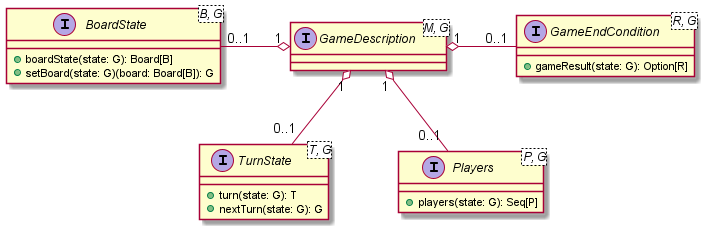
\includegraphics[width=\linewidth]{images/uml/extensions.png}
    \caption{Diagramma delle classi per le estensioni dello stato}
    \label{fig:extensions}
\end{figure}

\subsection{RuleSet e Dsl}

Si analizza ora il design di dettaglio relativo al \texttt{RuleSet} e al suo \textbf{DSL}.

Il \texttt{RuleSet} idendifica l'insieme delle regole che definiscono se, in un determinato stato, una \textit{move} è valida e in quale modo questa modifichi lo stato del gioco al momento della sua esecuzione.
%
La modalità con cui viene abilitato l'utilizzo del DSL, all'interno della definizione del proprio \texttt{RuleSet}, consiste nel dichiarare una classe (o un oggetto) che estenda dal trait \texttt{RuleSet} e aggiungere il trait \texttt{RuleSetBuilder} come mixin.
%
In questo modo, lo sviluppatore ha a disposizione una sintassi e un insieme di parole chiave definite dalla libreria.
%
La modalità scelta introduce per il team il problema di come organizzare le dichiarazioni delle parole chiave per fare in modo che la soluzione sia modulare e scalabile. % TODO
%
Il DSL, per questo motivo, è stato suddiviso in diverse componenti per mantenere un alto livello di modularità.
%
Ciascuna componente è stata poi unificata, tramite l'utilizzo dell'ereditarietà multipla, in un unico trait (\texttt{RuleSetBuilder}) per consentire all'utente di abilitare l'intera sintassi con una sola dichiarazione.

Le componenti individuate sono descritte nei seguenti paragrafi.

% \paragraph{MovesGeneration}
% Fornisce gli strumenti per dichiarare l'insieme di tutti i generatori di \textit{move} per poi raccoglierli ed utilizzarli in ogni fase del gioco per generare la sequenza di tutte le mosse disponibili in un dato momento.

% \paragraph{MovesExecution}
% \'E la componente che permette di definire in quale modo il \textit{GameState} vada aggiornato; mette a disposizione vari costrutti per aggiungere comportamenti e routine da eseguire al verificarsi di una data \textit{move} e permette, inoltre, di specificare azioni da eseguire prima e dopo l'esecuzione di mosse specifiche.

\paragraph{MovesGeneration e MovesExecution}
Rappresentano il punto di collegamento tra il DSL e il \texttt{RuleSet}, poichè accumulano le varie regole scritte all'interno del sorgente in un unico punto e lo rendono disponibile per essere utilizzato come implementazione dell'interfaccia del \texttt{RuleSet}.

\subparagraph{Generators}
Un \texttt{Generator} rappresenta l'astrazione di base utilizzata per la generazione delle mosse ed è costituito da una funzione che, partendo da uno stato di gioco, genera un certo insieme di mosse valide.
%
Tramite la componente \texttt{Generators} viene fornita all'utente la sintassi per la creazione dei generatori più comuni.

\subparagraph{Actions}
Come la \texttt{MovesGeneration} è fondata sul concetto di \texttt{Generator} come astrazione base, così la componente \texttt{MovesExecution} è fondata sul concetto di \texttt{Action}.
%
Una \texttt{Action} è rappresentata da una funzione che, a partire da uno stato, restituisce un nuovo stato.

Anche in questo caso, la componente \texttt{Actions} fornisce la sintassi per poter utilizzare le azioni più frequentemente impiegate nei giochi da tavolo.

\paragraph{Chainables and Modifiers}
Una volta forniti i mattoncini di base per la generazione e l'esecuzione delle mosse (rispettivamente \texttt{Generator} e \texttt{Action}), vengono forniti all'utente della libreria dei costrutti che consentono di combinare in diversi modi queste astrazioni.
%
Lo scopo è quello di permettere la creazione di azioni composite o di generatori più complessi, evitando di dover reinventare costantemente la ruota e riutilizzando il più possibile i meccanismi già implementati.

La soluzione fornita dalla libreria prevede la possibilità di \textbf{concatenare} tra di loro i meccanismi di base producendo nuove azioni o generatori, a loro volta combinabili. % TODO
%
Questa funzionalità è abilitata dalla type class \texttt{Chainable} (Figura \ref{fig:chainables}), che rappresenta una trasformazione \textbf{concatenabile} a un altra trasformazione dello stesso tipo. % TODO
%
\begin{figure}
    \centering
    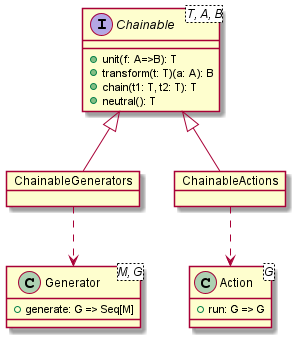
\includegraphics[width=0.5\linewidth]{images/uml/chainables.png}
    \caption{Diagramma delle classi contentente la struttura dei Chainable}
    \label{fig:chainables}
\end{figure}

Un tipo \texttt{Chainable} deve definire il modo in cui viene prodotto il risultato della concatenazione e deve inoltre definire il proprio \textbf{elemento neutro} (ovvero quello la cui concatenazione non ha effetto).
%
Quest'ultimo requisito consente di sfruttare il concetto di \texttt{Chainable} per permettere a generatori ed azioni di essere utilizzati all'interno di \textbf{costrutti iterativi e condizionali} (\texttt{Modifiers}).

\paragraph{Features}
Essendo il \texttt{RuleSet} definito a livello intensionale, è necessario avere un meccanismo per rappresentare le proprietà dello stato anche non avendo a disposizione una particolare istanza dello stesso.
%
Questa problematica è risolta dal concetto di \texttt{Feature}, ovvero una funzione che estrae dallo stato una sua proprietà.

La componente \texttt{Features} dichiara un insieme di \texttt{Feature} comunemente utilizzate.

\subsection{Interazione}

Le funzionalità abilitanti l'interazione con i giocatori sono state incapsulate totalmente nel modulo \texttt{interaction}, che comprende \texttt{view} e \texttt{controller}, con un interfacciamento verso il \texttt{model}.

Un gioco completo sviluppato con la libreria prevede due viste principali:
\begin{itemize}
    \item \textit{Menu}: il punto di ingresso dell'applicazione dove poter selezionare opzioni come giocare una nuova partita oppure uscire dal programma;
    \item \textit{Game}: una partita in corso.
\end{itemize}
%
Ciascuna di queste è composta da una specifica coppia di \texttt{subView} e \texttt{subController}.
%

% - View
\subsubsection{View}
% - - View principale -> Gestione subview
La \texttt{View} principale è in grado di creare e inizializzare le \texttt{SubView} esponendo un metodo per ritornare ognuna di esse: questo permette di centralizzare le informazioni relative al tipo della \texttt{View} e consente di rimpiazzarla in blocco. %brutto
% - - Menu view
\paragraph{Menu view} 
%
È il componente per gestire tutto ciò che è precedente o successivo al \textit{Game} (e.g. creazione \textit{Game}, chiusura dell'applicazione).
%
Il \texttt{MenuView} permette tramite un'apposita UI di scegliere come procedere tra le varie opzioni.
% - - Game view
\paragraph{Game view} 
%
È in grado di presentare il \textit{Game} nel caso di una \textit{move} valida, e in caso contrario gestisce la \texttt{Failure}.
%
Nello specifico, tramite la composizioni di \texttt{Renderer}, la \texttt{GameView} presenta la grafica dello stato attuale del \textit{Game}.
% - - - Renderers
\subparagraph{Renderer}
%
Compongono le \texttt{GameView} ed espongono un metodo per disegnare una specifica caratteristica del \textit{Game}.
%
Richiamando l'aggiornamento di tutti i \texttt{Renderer} la \texttt{GameView} è in grado di mostare tutte le caratteristiche dello stato attuale del \textit{Game}.
% - - - Event
\subparagraph{Event}
%
Rappresentano un'interazione dell'utente con la \texttt{GameView} e un'insieme di \texttt{Event} può comporre una \textit{move}.
%
Una \texttt{GameView}, in quanto \texttt{Observable}, è in grado di notificare il proprio \texttt{GameController} degli \texttt{Event} che vengono generati. 
% - Controller
\subsubsection{Controller}
I controller presentano una dipendenza dalle view in quanto devono chiamare i metodi della specifica \texttt{SubView} per fornire il feedback appropriato rispetto all'interazione intrapresa dal giocatore.
%
% - - Application controller
L'\texttt{ApplicationController} è responsabile di gestire la \texttt{View} principale, aggiungendovi i \textbf{listener} relativi e facendola partire.
% - - Menu controller
\paragraph{Menu controller}
%
Presenta le funzionalità per gestire l'avvio di una partita e la terminazione dell'applicazione.
%
Questo controller è una prima interfaccia con il \textbf{model}, che nel caso di avvio di una partita viene utilizzato nella forma della \texttt{GameDescription} per la generazione di un nuovo \texttt{Game}.
%
Successivamente viene preparata la GameView con i parametri relativi, viene aggiunto un nuovo \texttt{GameController} come listener e si passa alla nuova vista.
% - - Game controller
\paragraph{Game controller}
%
Gestisce gli \texttt{Event} che gli vengono notificati, presentando un comportamento diverso in base alla situazione:
\begin{itemize}
    \item Se l'evento assieme a quelli precedentemente salvati corrisponde ad una \texttt{Move}, allora questa viene eseguita sul \texttt{Game} e gli eventi memorizzati vengono azzerati;
    \item Se l'evento assieme a quelli precedentemente salvati non corrisponde ad una \texttt{Move}, allora viene memorizzato;
    \item Se l'evento è \texttt{Quit} allora termina la \texttt{GameView}.
\end{itemize}
\begin{itemize}
    \item Se l'evento assieme a quelli precedentemente salvati corrisponde ad una \texttt{Move}, allora questa viene eseguita sul \texttt{Game} e gli eventi memorizzati vengono azzerati;
    \item Se l'evento assieme a quelli precedentemente salvati non corrisponde ad una \texttt{Move}, allora viene memorizzato;
    \item Se l'evento è \texttt{Quit} allora termina la \texttt{GameView}.
\end{itemize}
